\documentclass{article}
\usepackage[a4paper, margin=2cm]{geometry} % Keep A4 paper and standard margins
\usepackage{tikz}
\usetikzlibrary{shapes.geometric, arrows.meta, positioning, fit}
\usepackage{lipsum} % Just for adding dummy text before/after diagram if needed

\begin{document}

% \lipsum[1] % Optional dummy text before

\begin{figure}[htbp]
\centering
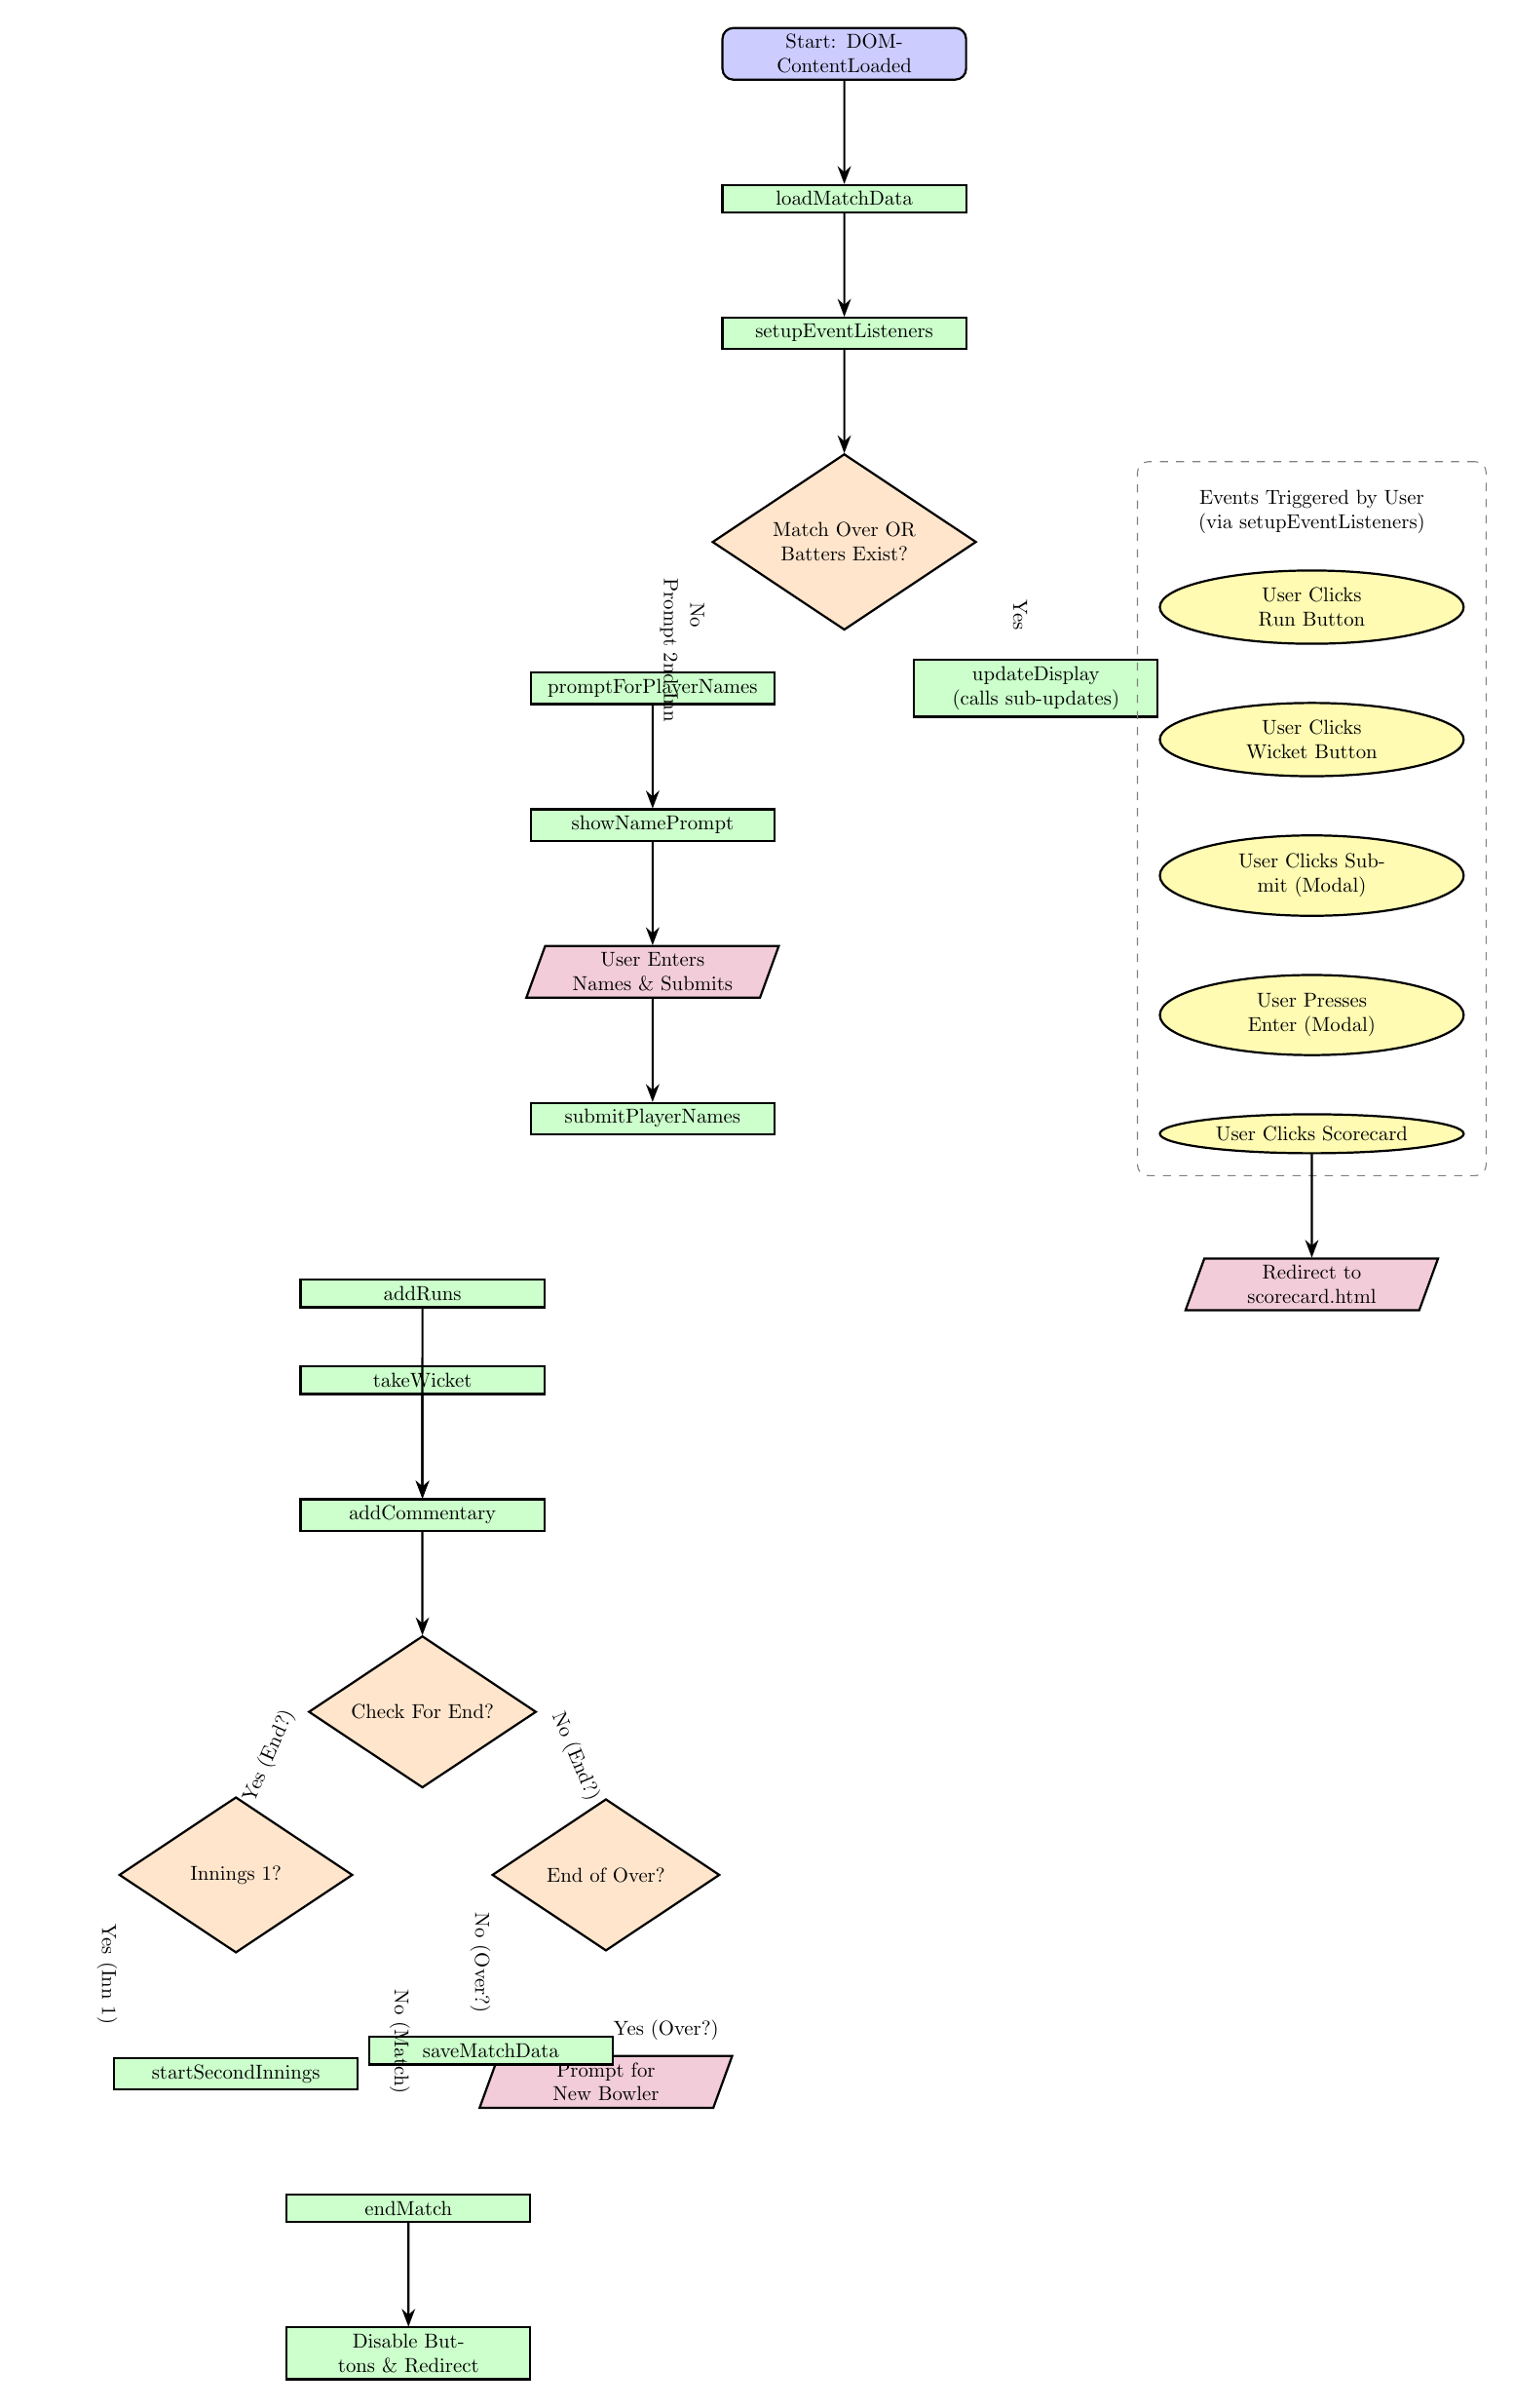
\begin{tikzpicture}[
    scale=0.75, transform shape, % Compromise scale (between 0.7 and 0.8)
    node distance=1.8cm and 1.2cm, % Reduced vertical, kept horizontal (from 2cm & 1.5cm)
    startstop/.style={rectangle, rounded corners, draw, fill=blue!20, thick, align=center, text width=4cm}, % Keep node styles allowing wrap
    process/.style={rectangle, draw, fill=green!20, thick, align=center, text width=4cm},
    decision/.style={diamond, draw, fill=orange!20, thick, aspect=1.5, align=center, text width=3cm},
    io/.style={trapezium, trapezium left angle=70, trapezium right angle=110, draw, fill=purple!20, thick, align=center, text width=3.5cm},
    event/.style={ellipse, draw, fill=yellow!30, thick, align=center, text width=3.5cm},
    arrow/.style={-Stealth, thick},
    line/.style={thick}
]

% --- Section 1: Initial Page Load & Setup --- (Layout unchanged)
\node (start) [startstop] {Start: DOMContentLoaded};
\node (loadData) [process, below=of start] {loadMatchData};
\node (setupListeners) [process, below=of loadData] {setupEventListeners};
\node (checkInitial) [decision, below=of setupListeners] {Match Over OR Batters Exist?};

% --- Section 2: Initial Branches (New Game vs Resume) --- (Layout unchanged)
\coordinate (checkInitialSouth) at ([yshift=-1cm]checkInitial.south); % Adjust coordinate slightly if needed

\node (promptNames) [process, left=of checkInitialSouth] {promptForPlayerNames};
\node (showPrompt) [process, below=of promptNames] {showNamePrompt};
\node (userInputNames) [io, below=of showPrompt] {User Enters Names \& Submits};
\node (submitNames) [process, below=of userInputNames] {submitPlayerNames};

\node (updateDisplay) [process, right=of checkInitialSouth] {updateDisplay (calls sub-updates)};

% --- Section 3: Event Trigger Nodes (Placement might need slight adjustment) ---
\coordinate (eventsAnchor) at ([yshift=-9cm]start.south); % Adjust vertical anchor if needed
\node (eventGroupLabel) [align=center, text width=4cm, right=6cm of eventsAnchor, yshift=1.5cm] {Events Triggered by User \\ (via setupEventListeners)};
\node (clickRun) [event, below=0.5cm of eventGroupLabel] {User Clicks Run Button};
\node (clickWicket) [event, below=1cm of clickRun] {User Clicks Wicket Button}; % Keep slightly reduced spacing here
\node (clickSubmitModal) [event, below=1cm of clickWicket] {User Clicks Submit (Modal)};
\node (pressEnterModal) [event, below=1cm of clickSubmitModal] {User Presses Enter (Modal)};
\node (clickScorecard) [event, below=1cm of pressEnterModal] {User Clicks Scorecard};
% Optional bounding box for events
\node [draw=gray, dashed, inner sep=8pt, rounded corners, fit=(eventGroupLabel) (clickRun) (clickWicket) (clickSubmitModal) (pressEnterModal) (clickScorecard)] {};

% --- Section 4: Gameplay Logic Nodes --- (Layout unchanged)
\coordinate (gameplayAnchor) at ([yshift=-1.5cm]submitNames.south); % Adjust anchor if needed
\node (addRuns) [process, below=1cm of gameplayAnchor, xshift=-4cm] {addRuns};
\node (takeWicket) [process, below=1cm of addRuns] {takeWicket};
\node (addCommentary) [process, below=of takeWicket] {addCommentary};
\node (checkEnd) [decision, below=of addCommentary] {Check For End?};

% --- Section 5: End Check Branches & Actions --- (Layout unchanged)
\coordinate (checkEndBelow) at ([yshift=-1.5cm]checkEnd.south); % Adjust coordinate slightly
\node (checkInning1) [decision, left=of checkEndBelow] {Innings 1?};
\node (startInning2) [process, below=of checkInning1] {startSecondInnings};

\node (checkOverEnd) [decision, right=of checkEndBelow] {End of Over?};
\node (promptBowler) [io, below=of checkOverEnd] {Prompt for New Bowler};

\node (endMatch) [process, below=of startInning2, xshift=3cm] {endMatch};
\node (endActions) [process, below=of endMatch] {Disable Buttons \& Redirect};
\node (redirectScorecard) [io, below=of clickScorecard] {Redirect to scorecard.html};

% --- Section 6: Shared Utility Nodes --- (Placement might need slight adjustment)
\coordinate (sharedNodeAnchor) at ([yshift=-1cm]startInning2.south |- checkEndBelow -| promptBowler.south); % Anchor lower down
\node (saveData) [process, below=of sharedNodeAnchor, xshift = -2cm] {saveMatchData}; % Position saveData lower


% --- Paths (Arrows) --- (Routing logic unchanged, distances adapt)
% Section 1 Flow
\path [arrow] (start) edge (loadData);
\path [arrow] (loadData) edge (setupListeners);
\path [arrow] (setupListeners) edge (checkInitial);

% Section 2 Branches
\path [arrow] (checkInitial.west) -- ++(-0.5,0) |- (promptNames) node[pos=0.25, above, sloped] {No};
\path [arrow] (checkInitial.east) -- ++(0.5,0) |- (updateDisplay) node[pos=0.25, above, sloped] {Yes};

\path [arrow] (promptNames) edge (showPrompt);
\path [arrow] (showPrompt) edge (userInputNames);
\path [arrow] (userInputNames) edge (submitNames);

% Section 3 Event Connections
\path [arrow] (clickRun) -| (addRuns);
\path [arrow] (clickWicket) -| (takeWicket);
\coordinate (submitNamesWest) at ([xshift=-1cm]submitNames.west);
\path [arrow] (clickSubmitModal.west) -- ++(-2,0) |- (submitNamesWest) -- (submitNames);
\path [arrow] (pressEnterModal.west) -- ++(-2,0) |- (submitNamesWest);
\path [arrow] (clickScorecard) edge (redirectScorecard);

% Section 4 Gameplay Flow
\path [arrow] (addRuns) edge (addCommentary);
\path [arrow] (takeWicket) edge (addCommentary);
\path [arrow] (addCommentary) edge (checkEnd);

% Section 5 End Check Branches
\path [arrow] (checkEnd.west) -- (checkInning1) node[midway, above, sloped] {Yes (End?)};
\path [arrow] (checkEnd.east) -- (checkOverEnd) node[midway, above, sloped] {No (End?)};

\path [arrow] (checkInning1.west) -- ++(-0.5,0) |- (startInning2) node[pos=0.25, above, sloped] {Yes (Inn 1)};
\path [arrow] (checkInning1.east) -- ++(0.5,0) |- (endMatch) node[pos=0.25, above, sloped] {No (Match)};

\path [arrow] (checkOverEnd.west) -- ++(-0.5,0) |- (saveData) node[pos=0.25, above, sloped] {No (Over?)};
\path [arrow] (checkOverEnd.south) |- (promptBowler) node[pos=0.25, right] {Yes (Over?)};
\path [arrow] (promptBowler) |- (saveData);

% Section 6 Connections to Shared Nodes
\path [arrow] (submitNames) |- (saveData);
\path [arrow] (startInning2) |- (saveData);
\path [arrow] (endMatch) |- (saveData);
\path [arrow] (endMatch) edge (endActions);

% Loop back paths
\coordinate (promptNamesNorth) at ([yshift=0.5cm]promptNames.north);
\path [arrow] (startInning2.west) -- ++(-1.5,0) |- (promptNamesNorth) -- (promptNames) node[pos=0.25, above, sloped] {Prompt 2nd Inn};

\coordinate (updateDisplaySouth) at ([yshift=-0.5cm]updateDisplay.south);
\path [arrow] (saveData.east) -- ++(2.5,0) |- (updateDisplaySouth) -- (updateDisplay);


\end{tikzpicture}
\caption{Flowchart of JavaScript Cricket Score Application Logic (Balanced A4 Layout)}
\label{fig:flowchart_a4_balanced}
\end{figure}

% \lipsum[2] % Optional dummy text after

\end{document}